\begin{figure}[!h]
    \centering
    \begin{subfigure}[t]{0.605\columnwidth}
        \centering
        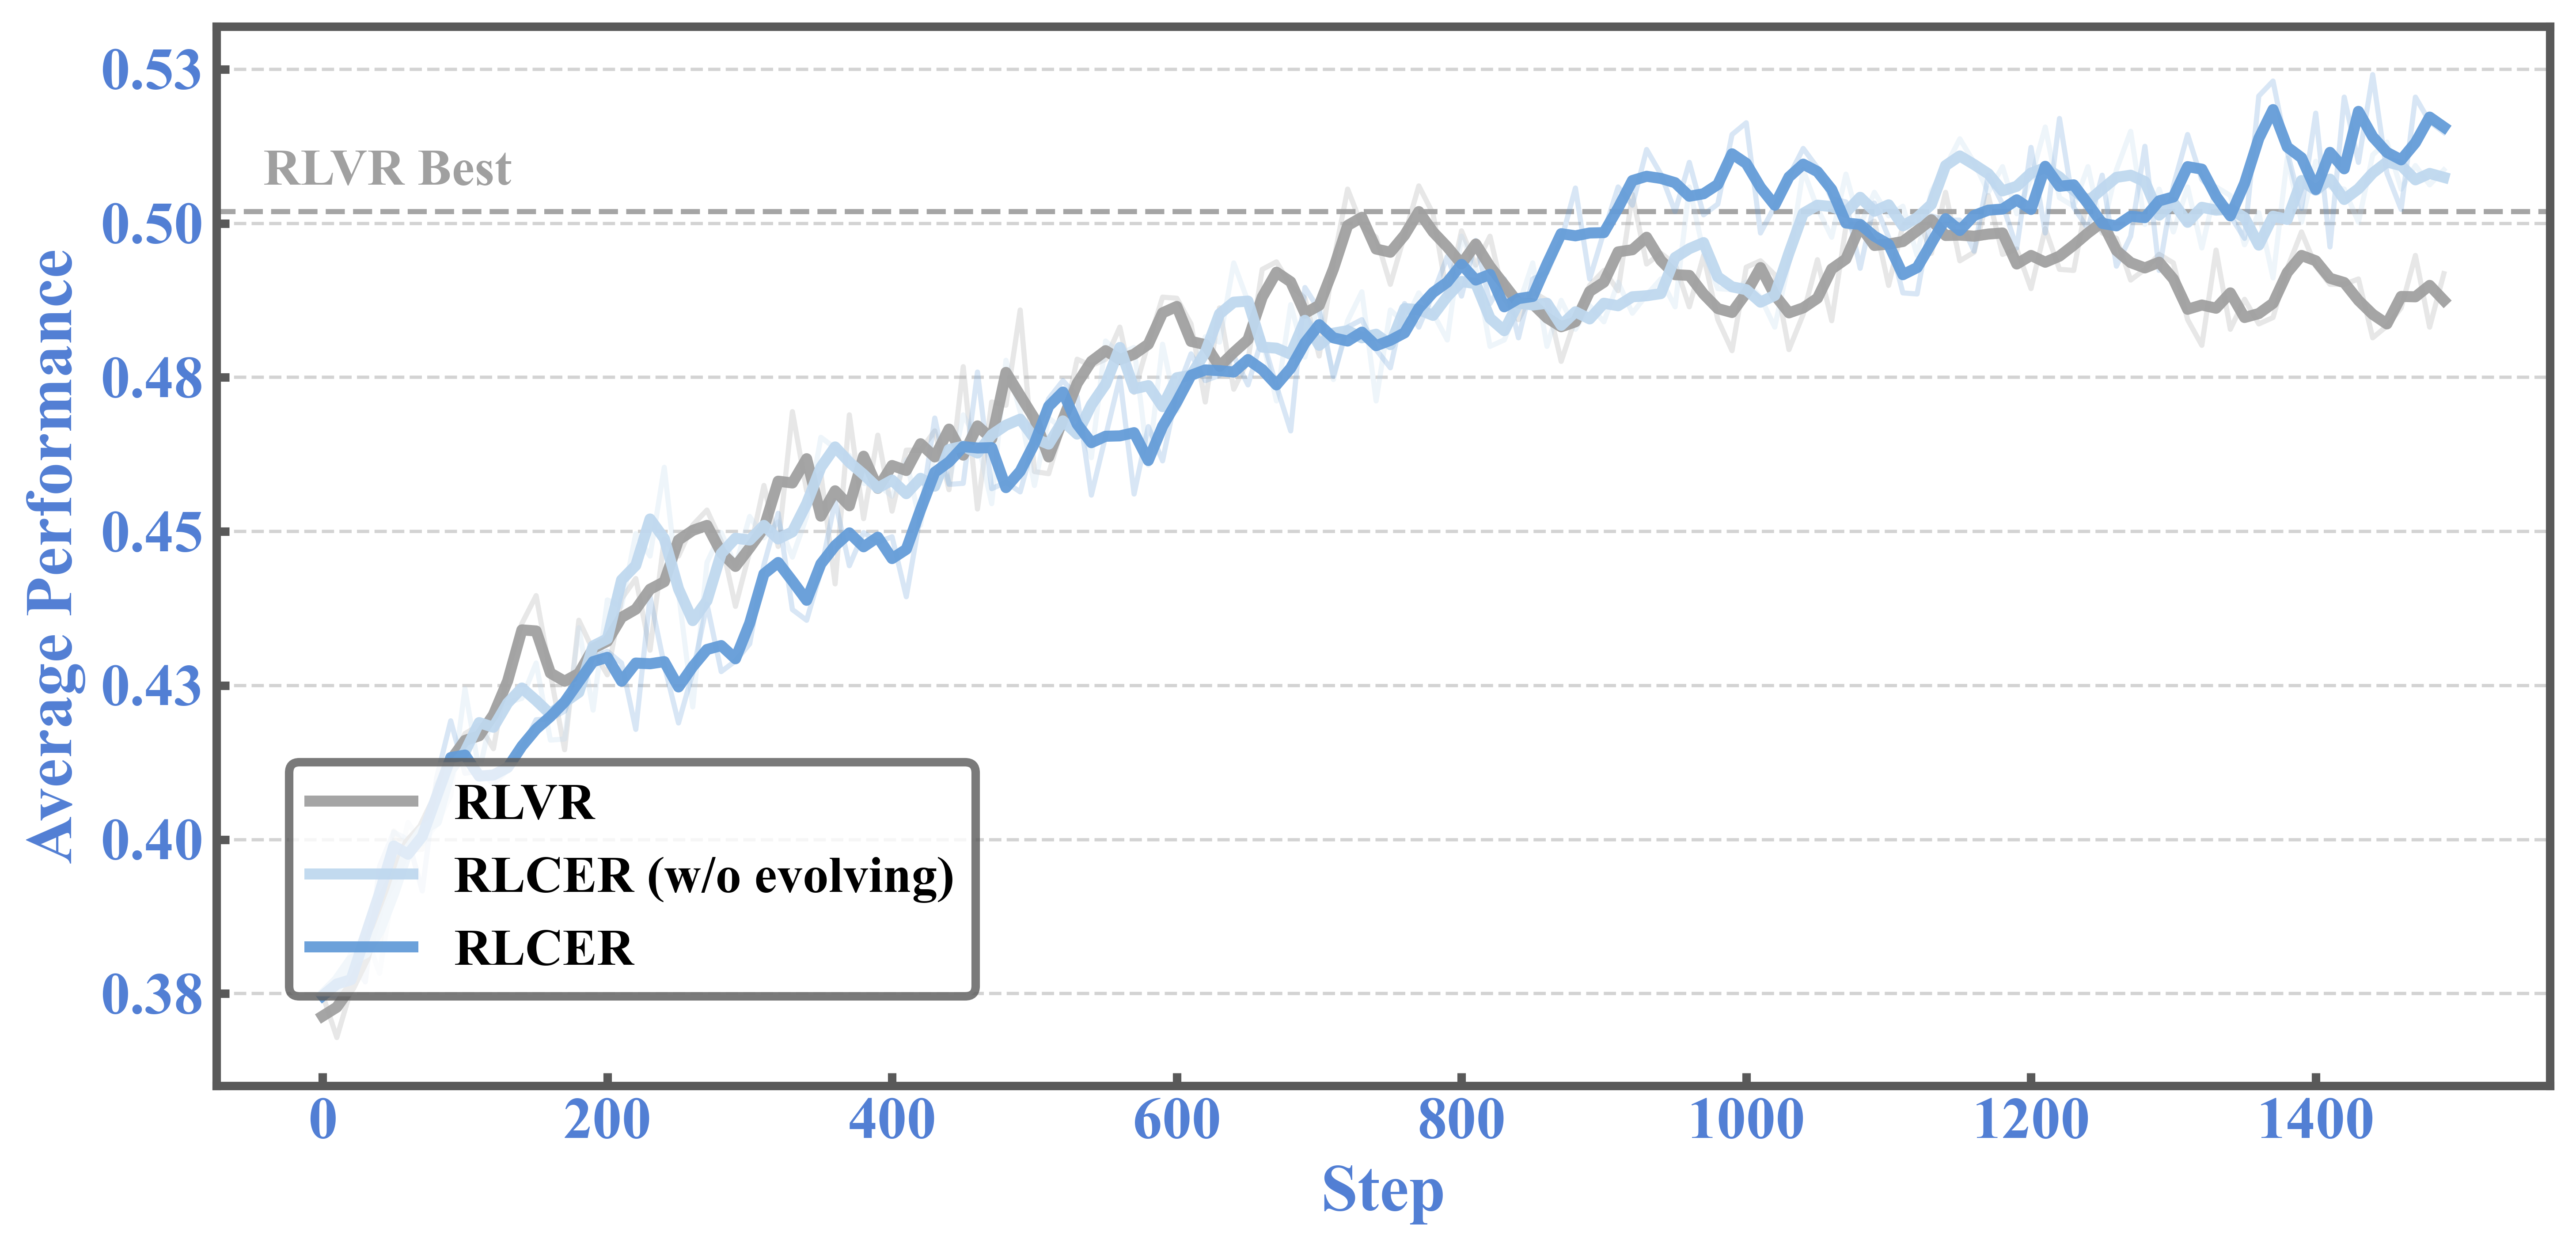
\includegraphics[width=\linewidth]{figures/exp/evolving_ablation/evolving_abl_perf.png}
        \vspace{-20pt}
        \caption{Average performance dynamics.}
        \label{fig:ablation-perf-dynamics}
    \end{subfigure}
    \begin{subfigure}[t]{0.382\columnwidth}
        \centering
        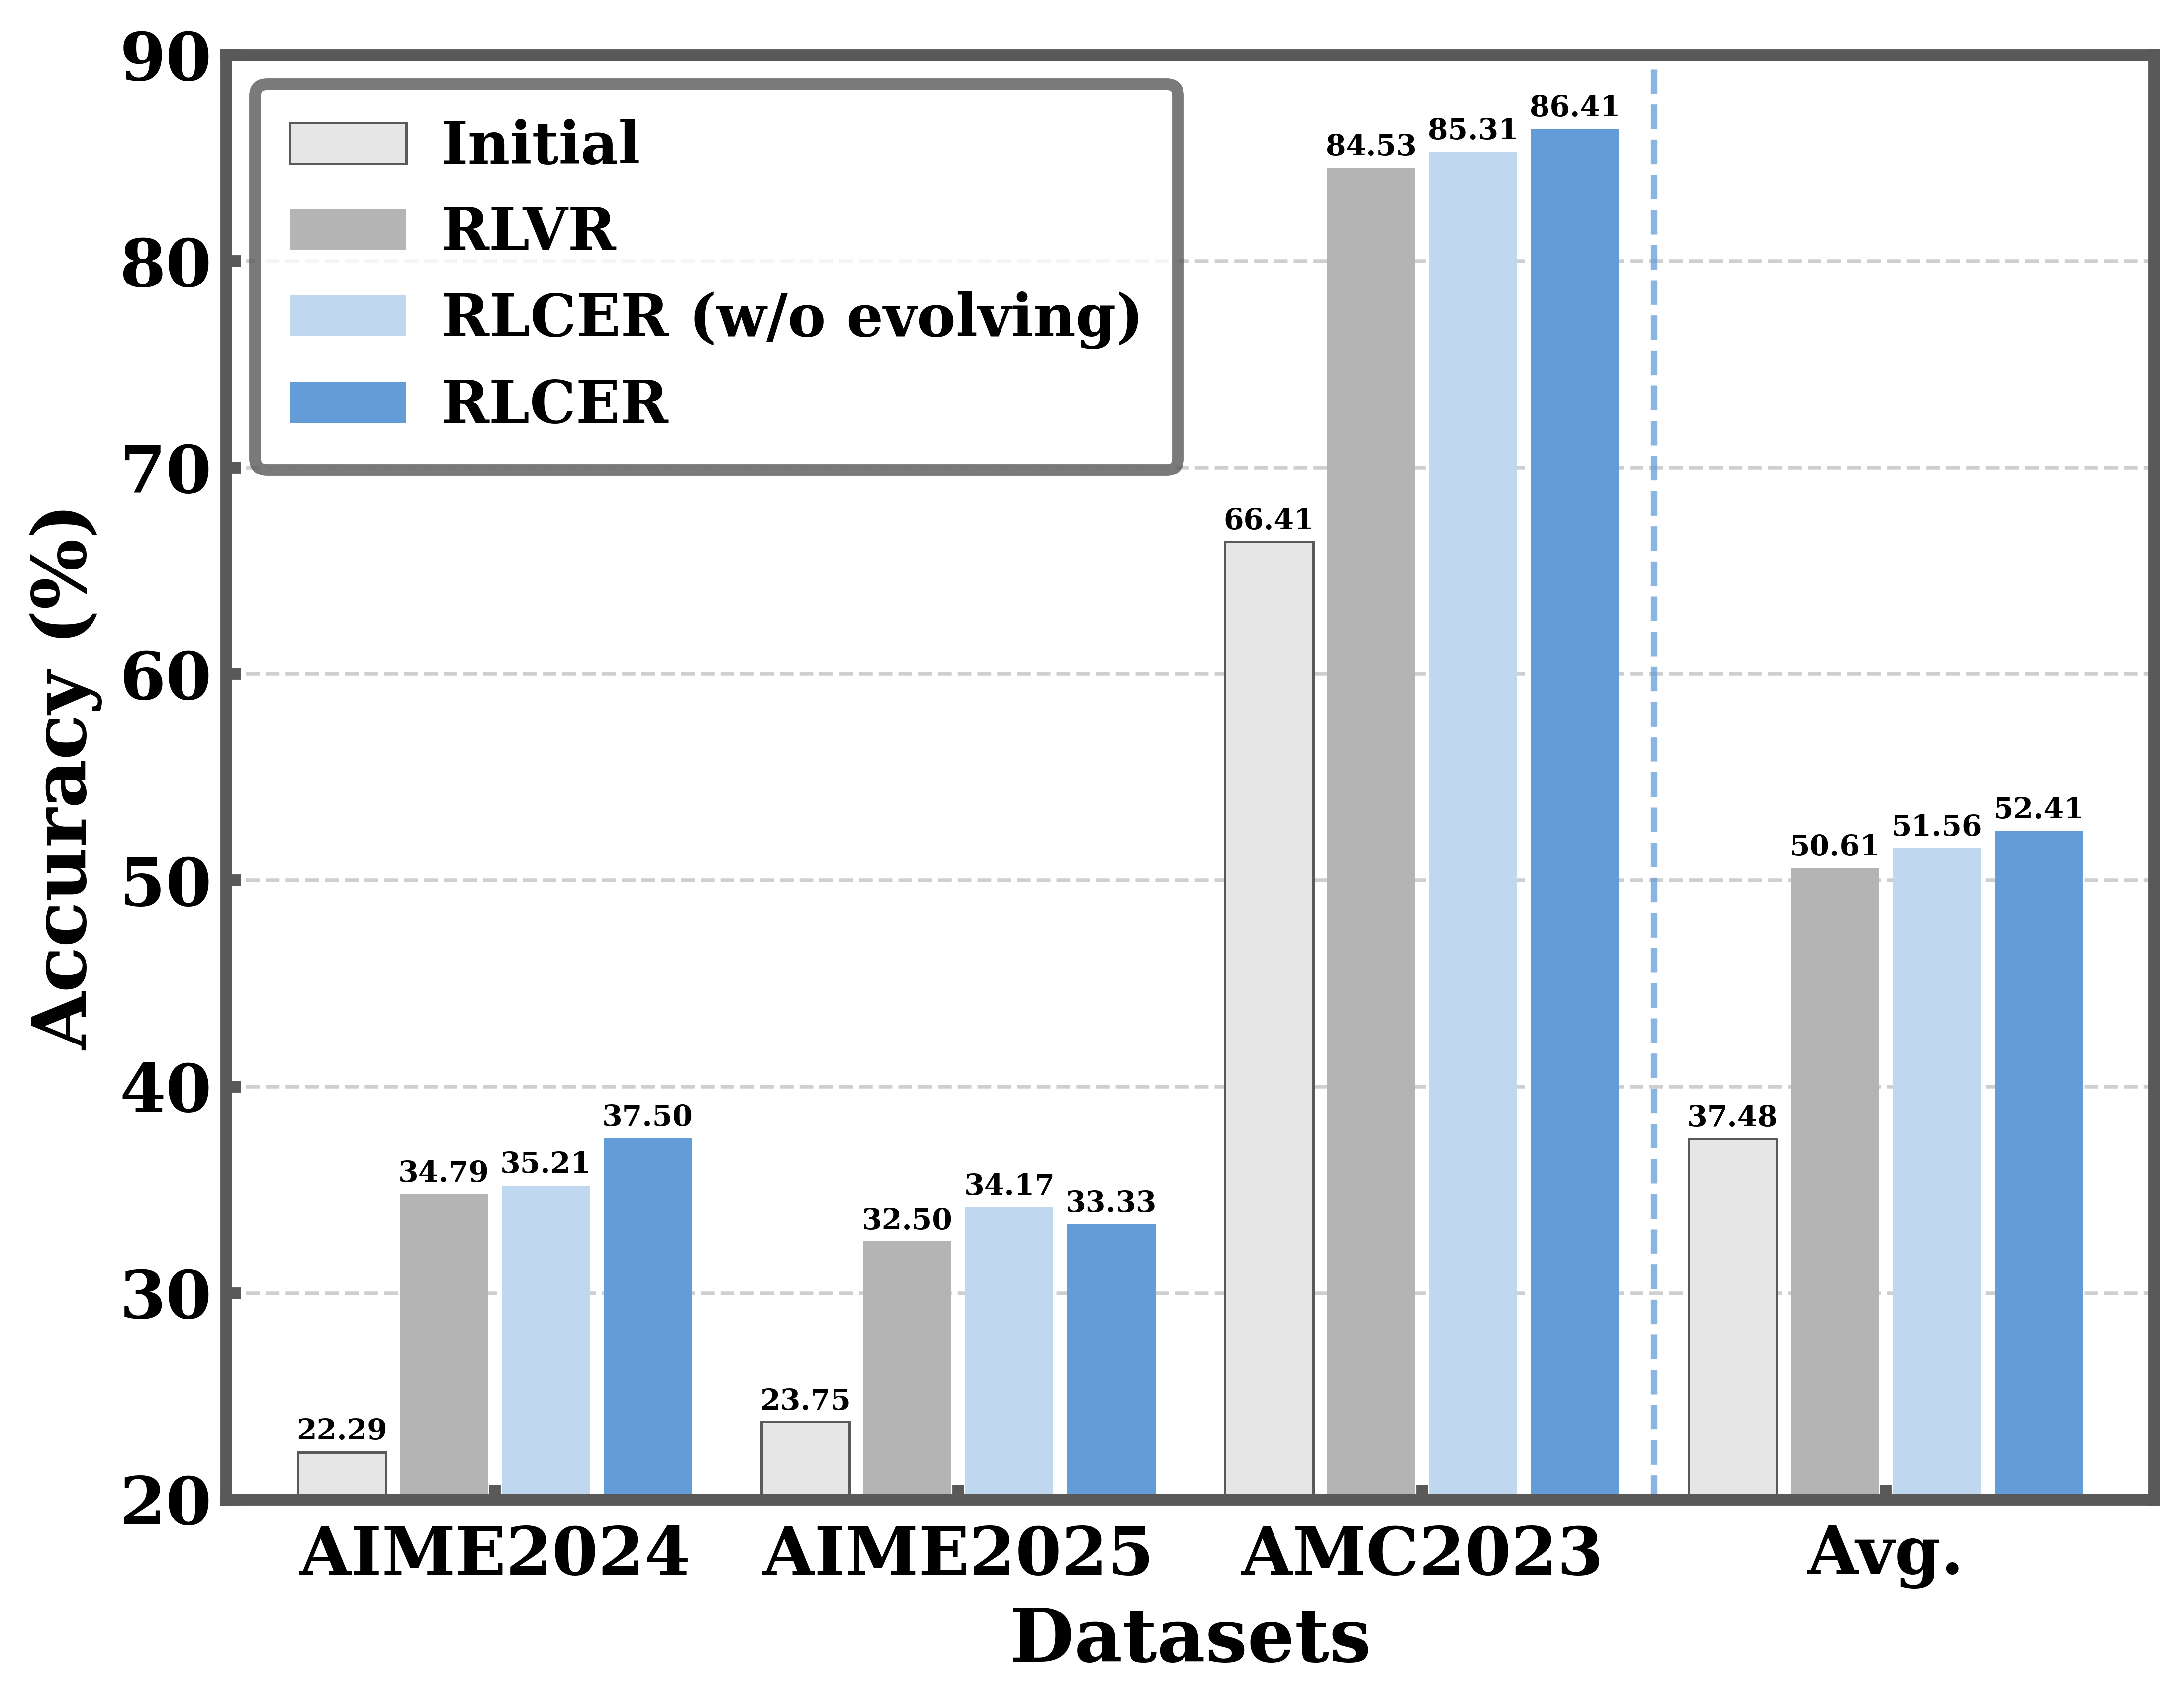
\includegraphics[width=\linewidth]{figures/exp/evolving_ablation/abl_perf.png} % ABLperf
        \vspace{-20pt}
        \caption{Performance comparison.}
        \label{fig:ablation-perf-final}
    \end{subfigure}
    \vspace{-8pt}
    \caption{Performance across three math datasets on the 7B model. Training with RLCER leads to a higher performance ceiling, and the self-evolving rubrics further enhance reasoning performance. }
    \label{fig:ablation-perf}
\end{figure}




\clearpage
\section{Introduction}


\begin{figure}[ht]
    \centering
    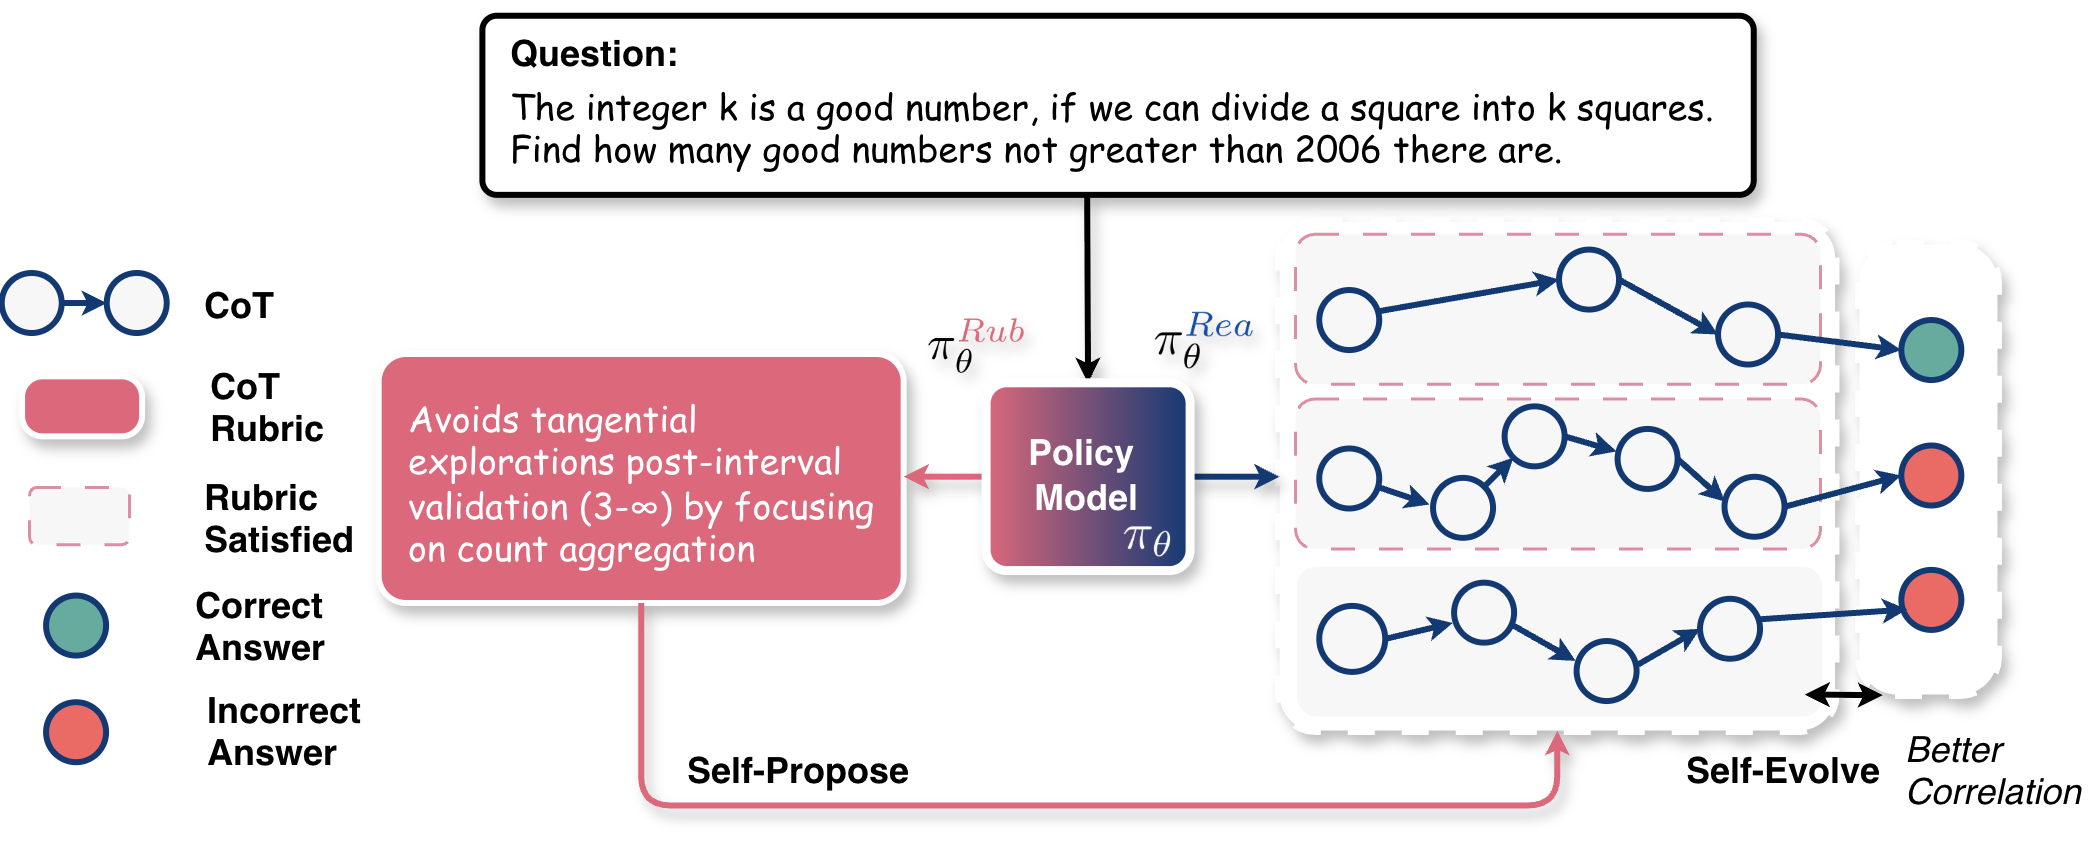
\includegraphics[width=0.9\columnwidth]{figures/framework/RLCER_teaser.png}
    \vspace{-8pt}
    \caption{Key idea of reinforcement learning with CoT supervision via self-evolving rubrics (RLCER). The policy model $\pi_\theta$ acts as both the reasoner and the rubrics generator, self-generating and self-evolving the rubrics for CoT supervision, where the evolving direction is shaped towards the correlation with the rubrics satisfaction and the final answer correctness.}
    \label{fig:teaser-figure}
    \vspace{-6pt}
\end{figure}


Chain-of-thought (CoT) \cite{CoT} reasoning is essential for large language models (LLMs) to solve complex tasks, where its quality strongly affects the final-answer correctness \cite{Demystifying-CoT, what-characterizes-cot, LCoT2Tree, ProcessBench}. 
However, CoT is rarely rewarded or optimized explicitly, even often regarded as a by-product of outcome-centric optimization objectives in large-scale reinforcement learning with verifiable rewards (RLVR) \cite{Deepseek-R1, O1, DeepSeekMath}.
This yields an underconstrained learning signal: for the same final answer, many distinct reasoning trajectories receive identical rewards, allowing optimization to drift toward shortcut or brittle strategies \cite{RuscaRL, zhang2025interplay}. Consequently, the model can converge to sub-optimal reasoning behaviors, limiting robustness and overall capability \cite{PRM8K}.

\revision{However, while important, directly rewarding or supervising CoTs remains challenging in practice, mainly for two reasons:}
(i) training additional reward models (RMs) for CoT supervision typically requires labor-intensive and fine-grained annotations \cite{PRM8K, PRIME}, 
and (ii) the policy’s CoT distribution shifts during training, yielding non-stationary and potentially biased supervision. 
\textit{\textbf{Can the policy model \concept{self-propose} rubrics as CoT supervision criteria and self-evolve them during training with no human annotations?}} 
If so, this could enable a new paradigm of self-improving reasoning, shifting RL from optimizing \concept{what LLMs answer} to autonomously improving \concept{how LLMs think}, potentially yielding \concept{``free-lunch''}  reasoning gains.

We find possibilities of achieving this from the recent advances in the research line of \concept{self-evolving training methods} \cite{self-evolving-survey, AlphaZero}, where a policy model $\pi_\theta$ can improve itself with little to no human intervention during training.
On the one hand, $\pi_\theta$ itself can self-generate training data, such as verifiable question-answer pairs for RL or high-quality CoT trajectories for cold-starting reasoning \cite{AbsoluteZero, SPICE, SSP, STaR}.
On the other hand, $\pi_\theta$ itself can self-assign reward signals by acting as a judge to evaluate its own solutions \cite{Self-Rewaring-Rubric, SRLM, SeRL, SPIN}.
A key idea shared by these methods is to let a single policy model $\pi_\theta$ play multiple roles under different prompts, serving not only as a reasoner that produces solutions but also as a data generator or a reward provider \cite{AbsoluteZero, SRLM}, with all roles optimized jointly (\eg via techniques such as multi-agent reinforcement learning \cite{AbsoluteZero}). 
Together, these capabilities make it plausible to self-propose supervision criteria (\eg rubrics) for assessing CoT quality and to self-evolve as training progresses.
However, how to adaptively propose and evolve such criteria in the self-evolving training paradigm remains largely underexplored.

To fill this gap, we propose \textbf{RLCER} (\textbf{R}einforcement \textbf{L}earning with \textbf{C}oT Supervision via Self-\textbf{E}volving \textbf{R}ubrics), empowering RLVR with self-proposed and self-evolving rubrics to supervise CoT reasoning.
The core idea is to let the policy model $\pi_\theta$ self-propose CoT supervision criteria as natural-language rubrics (\ie describing desirable reasoning properties like ``avoid tangential explorations'')
\cite{Rubrics-as-Rewards, Chasing-the-Tail}, rewarding CoTs by their rubric satisfaction, and simultaneously improving the model’s rubric-generation ability throughout training.
An overview of the key process is illustrated in Figure~\ref{fig:teaser-figure}.
Specifically, a single policy model $\pi_\theta$ is instantiated with different prompts to play two roles: a reasoner $\pi_{\theta}^{\text{\textcolor{reasoner}{$Rea$}}}$ that generates CoTs $\hat{\mathcal{C}}$ and final answers $\hat{\mathcal{A}}$, and a rubricator $\pi_{\theta}^{\text{\textcolor{rubricator}{$Rub$}}}$ that generates a set of candidate rubrics $\hat{\mathcal R} \triangleq \{\hat{\tau}_k\}_{k=1}^{K}$, where $K$ is the number of rubrics $\hat{\tau}_k$. 
The reasoner is rewarded by both the final answer correctness and the CoT quality, which is measured by satisfaction of all valid rubrics $\hat{\tau}^{valid}_k$. 
Here, we deem a rubric $\hat{\tau}_k$ valid if its satisfaction indicator $\mathbf v_k$ is strongly correlated with final-answer correctness $\mathbf z$ across multiple sampled rollouts for the same question $\mathcal Q$ (\ie $\mathtt{corr}(\mathbf v_k,\mathbf z)>\alpha$), since a high correlation means that satisfying the rubric aligns with producing correct answers. 
Additionally, we encourage the rubricator to self-evolve its rubric generation capability by rewarding the fraction of valid rubrics among its proposals
 (\ie $\frac{|\{\hat{\tau}^{valid}_k\}|}{K}$). 

Generally, RLCER enables RLVR to move beyond outcome-centric optimization by rewarding CoTs with supervision criteria that are self-proposed and self-evolved, without any human annotation.
We further conduct comprehensive experiments to examine the effectiveness of the proposed RLCER. 
First, we conduct a primary study showcasing that self-proposed rubrics can be reliable and learnable even when training is driven solely by rubric-based rewards, without any outcome reward (\cf Section \ref{sec:rubrics-reliability}). 
Based on this insight, RLCER generally outperforms the naive RLVR (\cf Section \ref{sec:main-performance}). 
Additionally, introducing self-evolving training for the rubricator further improves the reasoning performance (\cf Section \ref{sec:rubrics-self-evolving}).
Moreover, the generated rubrics can even serve as in-prompt hints to enhance reasoning at inference time (\cf Section \ref{sec:rubrics-as-hint}).
Overall, our results suggest a new paradigm in which models autonomously generate CoT supervision criteria to strengthen RL training, pointing toward more self-improving and self-evolving reasoning systems. 
